\renewcommand\labelitemi{-}
\renewcommand\labelitemii{$\circ$}
\renewcommand {\thesection}{\arabic{section}}

\chapter*{Introduction générale}
\addcontentsline{toc}{chapter}{Introduction générale}
    Dans un scénario réel, la règle dit que plus la surface de la route est confrontée
     à des changements de climat (entre le froid et le chaud) et avec un manque de soins, 
plus elle subit des dommages et affecte ensuite la vie des gens.
\begin{figure}[h!]
  \center
  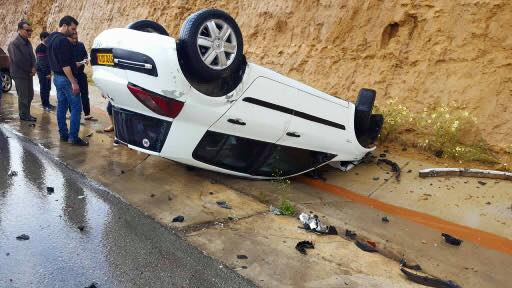
\includegraphics[width=0.75\textwidth]{Images/chapter1/accident.jpg}
 \caption{Accident de route}
 \label{fig:Accident}
  \end{figure}
Selon le centre national de prévention et de sécurité routière algérien : 
plus de 3.049 personnes avaient trouvé la mort et 29.095 personnes avaient été blessées
 dans 21.109 accidents enregistrés au niveau national lors des onze premiers mois de l'année 2019  \cite{nassimaAccidentsRouteAlger}.


\paragraph{} 
La surveillance de la surface des routes est un problème difficile dans le domaine des 
infrastructures de transport routier dans le monde entier. Une zone en mauvais état peut 
endommager les véhicules, les conducteurs et même provoquer un accident. 
Ils sont également à l'origine de poursuites et de dommages-intérêts coûteux, par exemple, 
en 2005, l'État du Michigan avait déposé plus de 7,500 réclamations pour dommages liés 
aux nids-de-poule \footnote{http://www.detnews.com/2005/specialreport/0510/18/A01-350197.htm}, et les 
compagnies d'assurance recevaient plus de 500,000 réclamations pour nids-de-poule chaque 
année\footnote{http://www.wktv.com/special/6733696.html}.

\section{Problématique}
Les municipalités du monde entier dépensent des millions de dollars pour entretenir et réparer leurs 
routes\footnote{http://boston.bizjournals.com/boston/othercities/denver/stories/2007/04/02/story1.html?b=1175486400\%5E1438887}.
 Malgré cet investissement, peu de gens sont satisfaits de la qualité de la route où ils vivent ou travaillent, car elles 
 réparent la surface sans étudier les véritables causes `` conditions '', tout comme la fermeture d'une plaie 
 sans la stériliser...\newline
 Ce qui maintient nos routes dans de bonnes conditions est un problème assez difficile
  en raison de nombreux facteurs tels que les intempéries, la charge de trafic imprévue et l'usure normale 
  dégradent toutes les routes même bien entretenues sur des périodes relativement courtes (semaines à mois).
% les conditions météorologiques difficiles et parce-que ils changent en fonction de la saison et de temps, ces derniers 
%causent des distorsions au niveau du la surface comme les bosses...

\section{Analyse de besoins}
Créer un outil pour mesurer la gravité de la route présente plusieurs problématiques. Avant de commencer le projet,  
 nous sommes amenés à répondre aux questions suivantes :
\begin{itemize}
	\item Quels sont ces différents facteurs et critères à prendre en compte pour prendre cette décision de mesure?
	\item Quelles sont les différentes difficultés et contraintes qui peuvent affecter cette décision?
	\item Peut-on offrir une solution informatique évoluée pour assister à cette décision? Si oui : 
        \begin{itemize}
            \item Comment mesurer Le niveau de médiocrité en route?
            \item Comment detecter/révéler les différentes causes d'une mauvaise route?
	      	  \item Comment localiser geographiquement chaque détections de ces causes?
	      	  \item Comment présenter cette solution aux usagers de manière simple et efficace ?
	      \end{itemize}
\end{itemize}

\section{Intérêts et avantages}
Développer un outil de route évolué a pour apport :
\begin{itemize}
	\item Un gain considérable de temps, efforts humains et une réduction de dépenses.
    \item Une surface de route soulide et surtout sans danger pour les piétons et les conducteurs.
    \item Une meilleure circulation en ville en diminuant le nombre d'accidents de route et ainsi réduire les
     dommages sur les véhicules.
\end{itemize}

\section{Clarification}
Dans nos recherches lors de l'étude du domaine problématique, nous observons que les anomalies
 les plus courantes sont les nids-de-poule (potholes) et les bosses(bumps).
  Ces deux catégories peuvent classer la plupart des anomalies trouvées dans notre vie quotidienne. Ainsi, nous avons:

  \subsection{les nids-de-poule}

Les nids-de-poule sont principalement causés par une mauvaise qualité de la chaussée ou des problèmes sous la surface.
\begin{figure}[h!]
  \center
  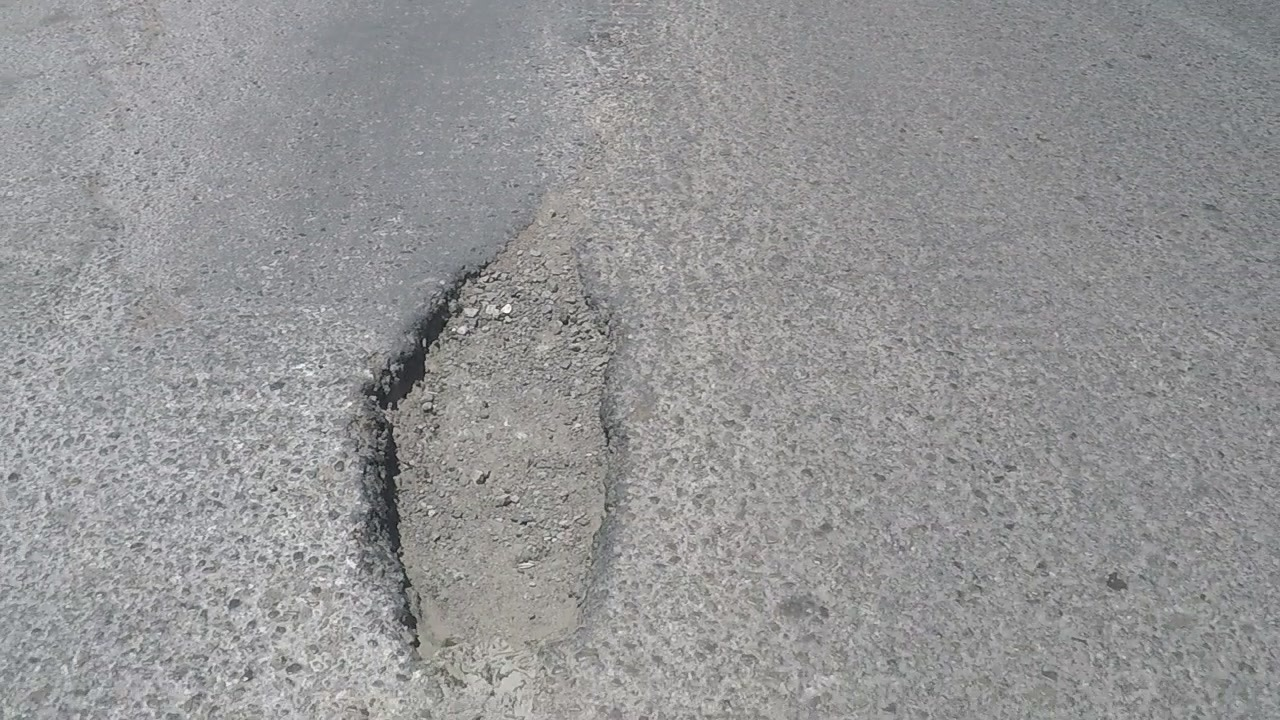
\includegraphics[width=0.4\textwidth]{Images/chapter1/Pothole.jpg}
  \caption{Nids-de-poule}
  \end{figure}
  \newline Un nid-de-poule est une dépression dans la surface d'une route, généralement une chaussée asphaltée, où la circulation 
a enlevé des morceaux cassés de la chaussée. 
C'est généralement le résultat de l'eau dans la structure du sol sous-jacente et du trafic passant sur la zone affectée.
 L'eau affaiblit d'abord le sol sous-jacent; le trafic fatigue et brise la surface asphaltée mal supportée de la zone touchée.
 L'action continue de la circulation éjecte l'asphalte et le sol sous-jacent pour créer un trou dans la chaussée.
\footnote{https://en.wikipedia.org/wiki/Pothole}

\subsection{ Les Ralentisseurs (longues et courtes)}

Normalement fabriquées par l'homme et généralement utilisées pour ralentir les véhicules à proximité des passages pour piétons.
\begin{figure}[h!]
    \center
    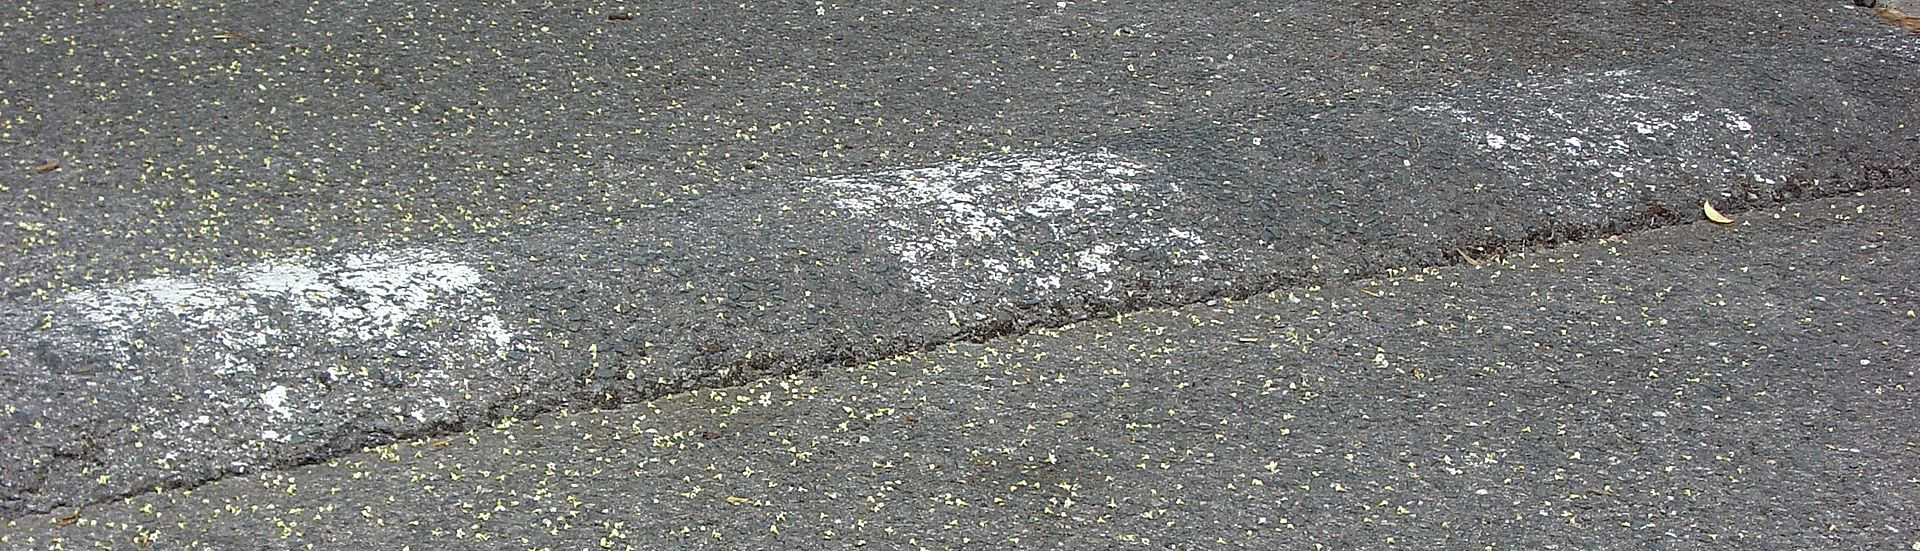
\includegraphics[width=0.9\textwidth]{Images/chapter1/Speedbump.jpg}
    \caption{Ralentisseurs}
    \end{figure}
On constate le plus souvent qu'ils imposent une limite de vitesse basse, inférieure à 40 km / h (25 mi / h) ou moins.
Bien que les ralentisseurs soient efficaces pour maintenir la vitesse des véhicules, leur utilisation est parfois 
controversée car:
 \begin{itemize}
    \item Ils peuvent augmenter le bruit de la circulation.
    \item Peuvent endommager les véhicules s'ils sont traversés à une vitesse trop élevée et ralentir les véhicules d'urgence.
    \item Les ralentisseurs mal conçus qui se tiennent trop haut ou avec un angle
      trop aigu peuvent perturber les conducteurs et peuvent être difficiles à naviguer pour les véhicules à faible garde au sol,
      même à très basse vitesse.De nombreuses voitures de sport ont ce problème avec de tels ralentisseurs. 
    \item Les ralentisseurs peuvent également présenter de graves dangers pour les motocyclistes et les cyclistes s'ils ne sont pas
    clairement visibles, bien que, dans certains cas, une petite coupure sur le pare-chocs permette à ces véhicules de
     traverser sans obstacle.
  \end{itemize}

  Les ralentisseurs coûtent entre 50 et 200 Dolar et peuvent devoir être remplacés au fil du temps 
   en raison de l'usure 
   \footnote{https://en.wikipedia.org/wiki/Speed\_bump \newline *les ralentisseurs= bosses (i.e bump) *Les nids-de-poule = trou routière (i.e potholes)}.  


\section{Applications similaires}  
Pour ce projet, et en raison des conditions routières dans notre zone géographique (Algérie), nous avons décidé de ne nous concentrer que 
sur deux types d'anomalies: les bosses longues et courtes et les nids de poule.\newline
Ainsi une grande vague d'un travail riche et divers a commencé juste pour estimer et étudier les revêtements routiers pour l'améliorer.

\subsection{Une approche utilisant des caméras fixes : }
Cette méthode \cite{kawaiMethodDistinguishRoad2012} distincte  les conditions de surface de la route dans la nuit en utilisant une caméra montée sur une voiture.
En conséquence, elle est basée sur des caractéristiques d'image telles que la "luminance" et la "caractéristique de texture". 
Ils utilisent également les «informations de couleur» afin de prendre en compte l'existence de réverbères et de lampes de signalisation. De cette façon, il a été possible de distinguer les zones routières avec précision, y compris les parties éclairées par les lampadaires et autres sources de lumière en utilisant des informations de couleur. En conséquence, il a été possible d'obtenir une précision de distinction de 96 \% sur sec, 89\% sur mouillé et 96\% sur neige.
L'un des problèms avec cette methode le coût des appareils où il est élevé, de plus, les cibles d'estimation sont limitées aux routes qui ont des dispositifs fixes .
\begin{figure}[h!]
    \center
    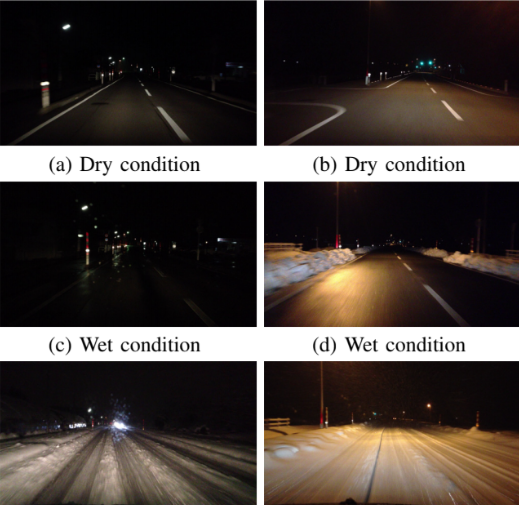
\includegraphics[width=0.45\textwidth]{Images/chapter1/cameraFixe.jpg}
    \caption{Utilisation des cameras fixes}
    \end{figure}
   
\subsection{Une approche utilisant des black-box cameras :}

    Cette approche \cite{joPotholeDetectionSystem2015} propose un nouveau système de détection de nids de poule utilisant une caméra à boîte noire commerciale. Le but de cette recherche est de développer un détecteur de nids-de-poule en utilisant des dispositifs communs qui sont utilisés par de nombreux conducteurs sur une large zone. De plus, les dispositifs devraient fournir une précision de détection élevée à faible coût. L'appareil le plus approprié pour cette exigence est la caméra à boîte noire où ils installent leur algorithme de détection des nids-de-poule, de sorte que tous les véhicules sur les routes seront un détecteur de ces derniers.
    \begin{figure}[h!]
      \center
      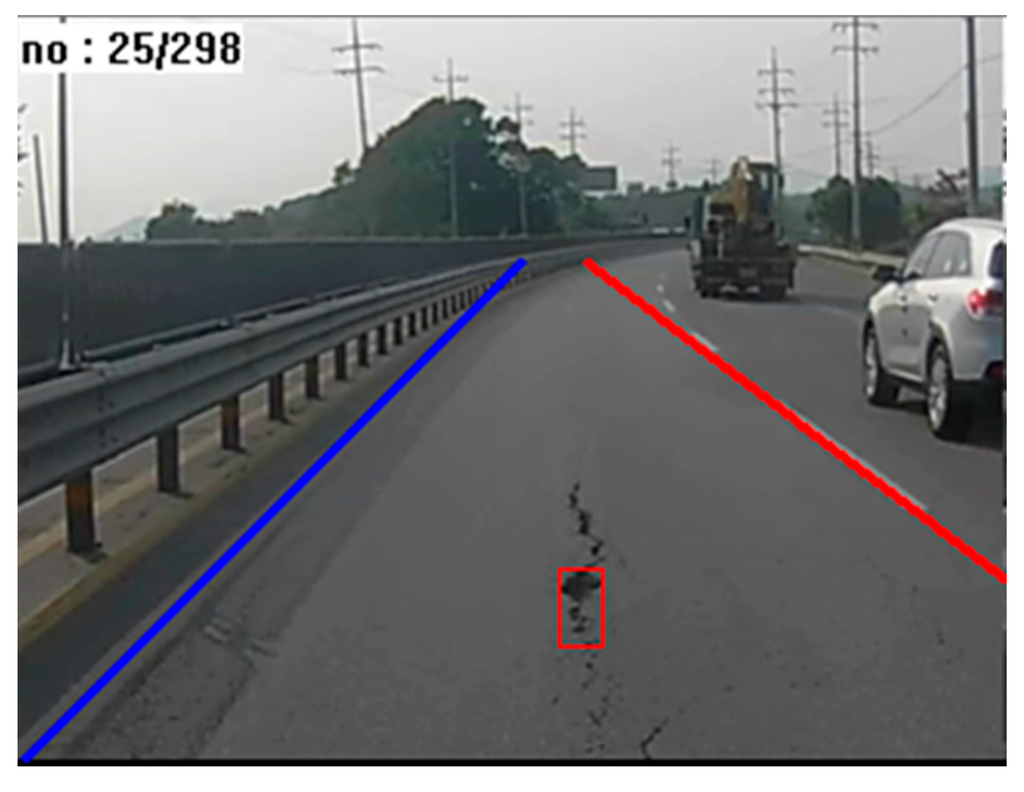
\includegraphics[width=0.51\textwidth]{Images/chapter1/resultatDePotholDetection.jpg}
      \caption{Resultat d'une detection de nid-de-poule}
      \end{figure}



\chapter*{La detection mobile <<Mobile sensing>>}
\addcontentsline{toc}{chapter}{La detection mobile <<Mobile sensing>>}
Récemment, des petits capteurs hautes de performances se sont répandus et sont intégrés dans divers types d'objets dans notre environnement.\newline
La détection mobile "Mobile sensing" utilise des capteurs intégrés dans des objets en mouvement tels que des voitures, des vélos et des smartphones, et les considère comme des capteurs de detection \cite{nomuraMethodEstimatingRoad2015}.\newline
De plus, le taux de pénétration des smartphones de haute qualité augmente et continuera de le faire. Ces derniers incluent de différents types de capteurs tels que des capteurs d'accélération et des capteurs gyroscopiques.

%---- talking about sensors---%


\section{Capteurs d'un smartphone} 

Le capteur est un appareil qui détecte les changements dans l'environnement proche et envoie ces données au système d'exploitation ou au processeur. Ils détectent et collectent les données pour lesquelles ils sont faits.\newline
Il existe trois catégories principales de capteurs que possède un smartphone \cite{tilluMobileSensorsComponents2019}.

\subsection{Les capteurs de mouvements:}
 ils mesurent les forces d'accélération et les rotations autour des trois axes.  Ces capteurs sont capables de déterminer dans quelle direction est orienté l’appareil. A titre d’exemple, On trouve l'accéléromètre, les capteurs de gravité, les gyroscopes et les capteurs de vecteurs de rotation.

 \subsection{Les capteurs de position et d’attitude:}
  Ce genre de capteurs détermine la position et l’orientation de l'appareil. On trouve donc les capteurs d’orientation, le gyroscope et le magnétomètre ainsi que le GPS. 
 
 \subsection{Les capteurs environnementaux:}
 c’est des capteurs qui mesurent la pression atmosphérique, l'illumination et la température ambiante. (Baromètre, photomètre et thermomètre).

 \section{Définitions} 

 \subsection{Accéléromètre}
 L'accéléromètre détecte la détection de mouvement basée sur l'axe. Il détecte les changements d'orientation des smartphones par rapport aux axes x, y et z.Cette accélération est utilisée pour déterminer la vitesse de l’appareil. La vitesse peut être intégrée pour déterminer le changement du périphérique de position et avec l’accélération on peut calculer l’orientation du smartphone.

 \subsection{Gyroscope}
Le gyroscope ou capteur gyroscopique est une version avancée de l'accéléromètre. Alors que l'accéléromètre détecte la détection de mouvement basée sur l'axe, le gyroscope fonctionne avec l'accéléromètre et détecte chaque degré de changement d'orientation. Il fournit une détection de mouvement très précieuse.

\subsection{GPS}
Le GPS ou le système de positionnement global est également très courant dans populaire est la plupart des téléphones modernes. Il aide à localiser l'emplacement sur Terre et aide à la navigation.


\section{La detection mobile avec des smartphones}

Avec cette évolution dans le domaine des mobiles, il est possible de développer un système pratique et efficace à faible coût et recueilli divers types d'informations afin de détecter les anomalies routières telles que les ralentisseurs et les nids de-poule.

\subsection{Détections des ralentisseurs}
Il existe des études sur la détection des ralentisseurs à l'aide de capteurs d'accélération \cite{nomuraMethodEstimatingRoad2015},il est basé sur une analyse itérative de plusieurs corps en utilisant un modèle de véhicule à plusieurs corps. La méthode \cite{nomuraMethodEstimatingRoad2015} utilise des capteurs d'accélération à trois axes et un capteur GPS intégrés dans un véhicule.\newline
La méthode \cite {nomuraMethodEstimatingRoad2015} consiste à placer un smartphone sur le tableau de bord d'une voiture et ne peut détecter les ralentisseurs que pendant la conduite,cette étude propose une méthode d'estimation de la hauteur et de la longueur des ralentisseurs à l'aide de capteurs d'accélération,apres elle estime la quantité de déplacement vertical en utilisant le double entier de la composante verticale des valeurs d'accélération, et la définit comme la hauteur de le ralentisseur. cette méthode permet d'estimer rapidement l'état de la chaussée à faible coût en utilisant des smartphones. Cependant, les ralentisseurs qui ne font pas ressentir des vibrations aux autres passagers ne sont pas détectées et les ralentisseurs qui font ressentir les vibrations aux autres passagers ne sont pas détectées.\newline
Par conséquent cette méthode a un problème de un problème de une détection inadéquate des changements dans l'état de la surface des routes "un problème de précision".

\section{Solution proposée}
Au moment de rédiger ce mémoire, aucune application en Algérie n’offre ce genre de service .
De ce fait, Nous proposons un outil permettant de :
\begin{itemize}
	\item Fournir à la direction des traveaux public "DTP" un moyen de se renseigner en temps réel sur la qualité des routes afin d'intervenir efficacement et le plus rapidement possible dans les travaux d'entretien.Ce qui permettra d’améliorer les manquements cités plus haut.
  \item Mieux assister le conducteur dans sa conduite en prévenant des ralentisseurs/dégradations de la route, afin de ralenir convenablement. \newline
  \item 
\end{itemize}
Pour cela, nous proposons de développer un système qui proposera les fonctionnalités suivantes :
\begin{itemize}
  \item Détecter les événements (les nids-de-poule et les ralentisseurs dans notre cas) en temps réel.La collecte de données brutes pour un post-traitement hors ligne est classée comme une fonctionnalité supplémentaire. 
  \item Utiliser un téléphone intelligent générique basé sur Android-OS avec des capteurs accéléromètres comme plate-forme matérielle / logicielle. La portabilité vers d'autres plates-formes est classée comme une fonctionnalité supplémentaire.
  \item Pouvoir fonctionner sur différents modèles de smartphones avec différents paramètres. Au cours du processus de mise en œuvre du système, l'ensemble des paramètres minimaux du smartphone doit être déterminé et décrit.
  \item Détecter les événements lors de la conduite dans différents types de véhicules à quatre roues tels que des voitures particulières, des mini-fourgonnettes et des bus. Les véhicules à deux roues tels que les motos et les scooters ne sont pas pris en compte.
\end{itemize}

\renewcommand {\thesection}{\thechapter.\arabic{section}}













